\subsubsection{Jobs}
\label{view_jobs}

\paragraph{}
The Jobs page, accessible via the session tab in the default navigation bar, lists jobs the user currently has waiting in the job queue, as illustrated in figure \ref{fig:view_jobs}. The user can delete jobs from the queue (resulting in the deletion of any downstream pending jobs and dafiles). They can also download the script which has been generated for the job.

\begin{figure}[h]
\centering
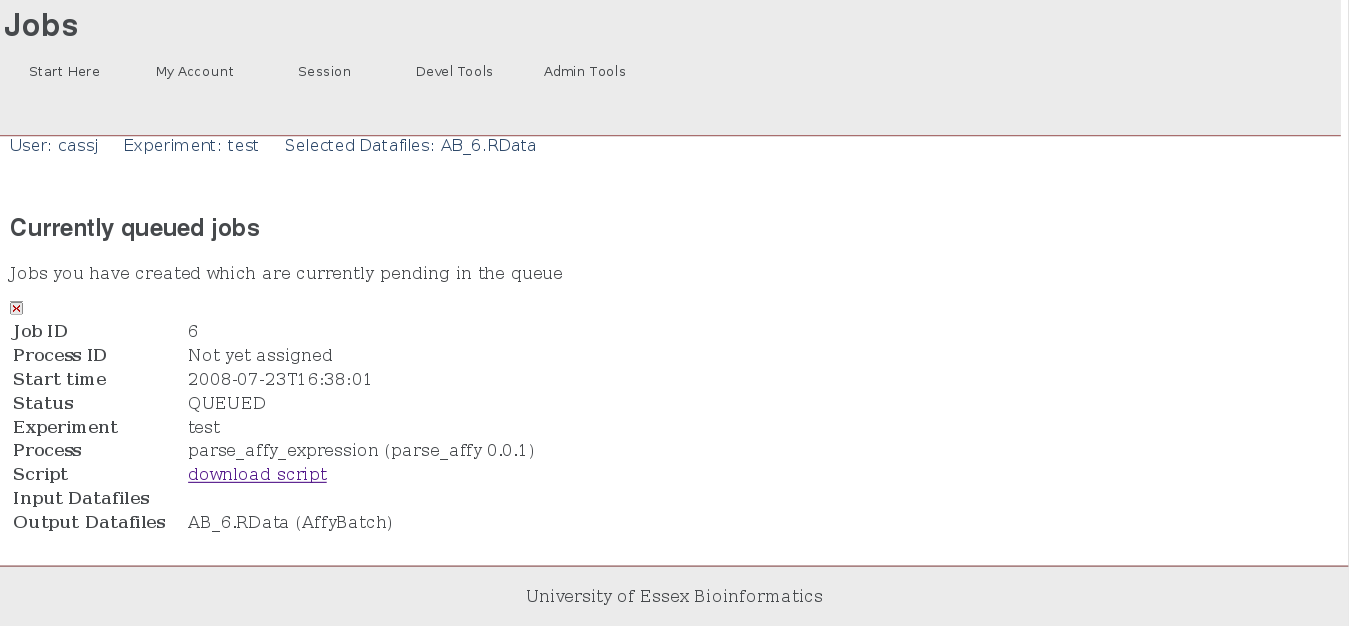
\includegraphics[scale=0.45, angle=90]{../rome/docs/images/screenshots/jobs}
\caption{The Job Queue}\label{fig:view_jobs}
\end{figure}

%To do: should be able to get previously run jobs. maybe link from the names of the edges in the datafile graph?